\section{Theoretical formalism of the \psq spectrum}
\label{sec:swave:theo}

The \BdToKpill angular distribution can be expressed for multiple S-wave states 
as described in Section~\ref{sec:fullangdist} and Ref.~\cite{Lu:2011jm}.
For \kpi masses below  
$1200\mev$,  the %it can be seen from the previous section that
contribution to the amplitudes from the higher $\Kstarz$ states is 
small enough that it can be ignored.
In order to understand the S-wave contribution to the \BdToKpill angular distribution
 close to the $\Kstarz(892)$ so only the $J=0,1$ terms in
the sums of Eq.~\ref{eq:amp} were considered.

The S-wave contribution to these amplitudes only enters in the amplitude $\mathcal{A}_{0}$, 
\begin{align}
\label{eq:amps1}
\mathcal{A}_{H0} &= \sqrt{\frac{1}{4\pi}} A_{0H0} + \sqrt{\frac{3}{4\pi}} A_{1H0} \ctk    \\
\mathcal{A}_{H||} &= \sqrt{\frac{3}{8\pi}} A_{1H||} \stk  \\
\mathcal{A}_{H\bot} &= \sqrt{\frac{3}{8\pi}} A_{1H\bot} \stk   
\end{align}
where the spherical harmonics are expanded, leaving the phase space factor, 
the propagator and the matrix element as part of the spin-dependent amplitudes
\begin{equation}
\label{eq:amps2}
\begin{split}
A_{0,H,0} &\propto \rho(\psq,\qsq) \times M_{0,H,0} (\qsq) \times  P_0(\psq) , \\
A_{1,H,0} &\propto  \rho(\psq,\qsq) \times  M_{1,H,0} (\qsq) \times  P_1(\psq) , \\
A_{1,H,\bot} &\propto  \rho(\psq,\qsq)  \times M_{1,H,\bot} (\qsq) \times  P_1(\psq) , \\
A_{1,H,||} &\propto  \rho(\psq,\qsq) \times M_{1,H,||} (\qsq) \times P_1(\psq) ,  
\end{split}
\end{equation}
where the first index denotes the spin. 
The normalisation from the three-body phase space factor is described in more detail below.

\subsection{Phase space factors}
\label{sec:swave:phasespace}

The phase space for the four-body decay \BdToKpill can be described by three three-body phase space factors
\begin{align}
\rho(\Bd\to(\kpi)(\ellell)) \times \rho((\kpi)\to\kaon\pion) \times \rho((\ellell)\to\ellp\ellm) \, .
\end{align}
The three-body phase space factor is
\begin{align}
\rho(a \to b c ) = \left(\frac{\sqrt{ \lambda ( a, b , c ) }}{8\pi a^2}\right)^{2J+1}
\end{align}
where $\lambda(a,b,c) = \left(a^2+b^2+c^2\right)^2-4b^2c^2$ is the triangle function and $J$ is
 the difference in spin of $a$ and $b$. 
%The \qsq-dependent phase space factor is assumed to be fixed and the combination of \qsq and \psq dependence is not considered in this chapter.
The phase space for \BdToKpill as a function of \psq and \qsq is given in Fig.~\ref{fig:phasespace}. 
\begin{figure}[tb]
\centering
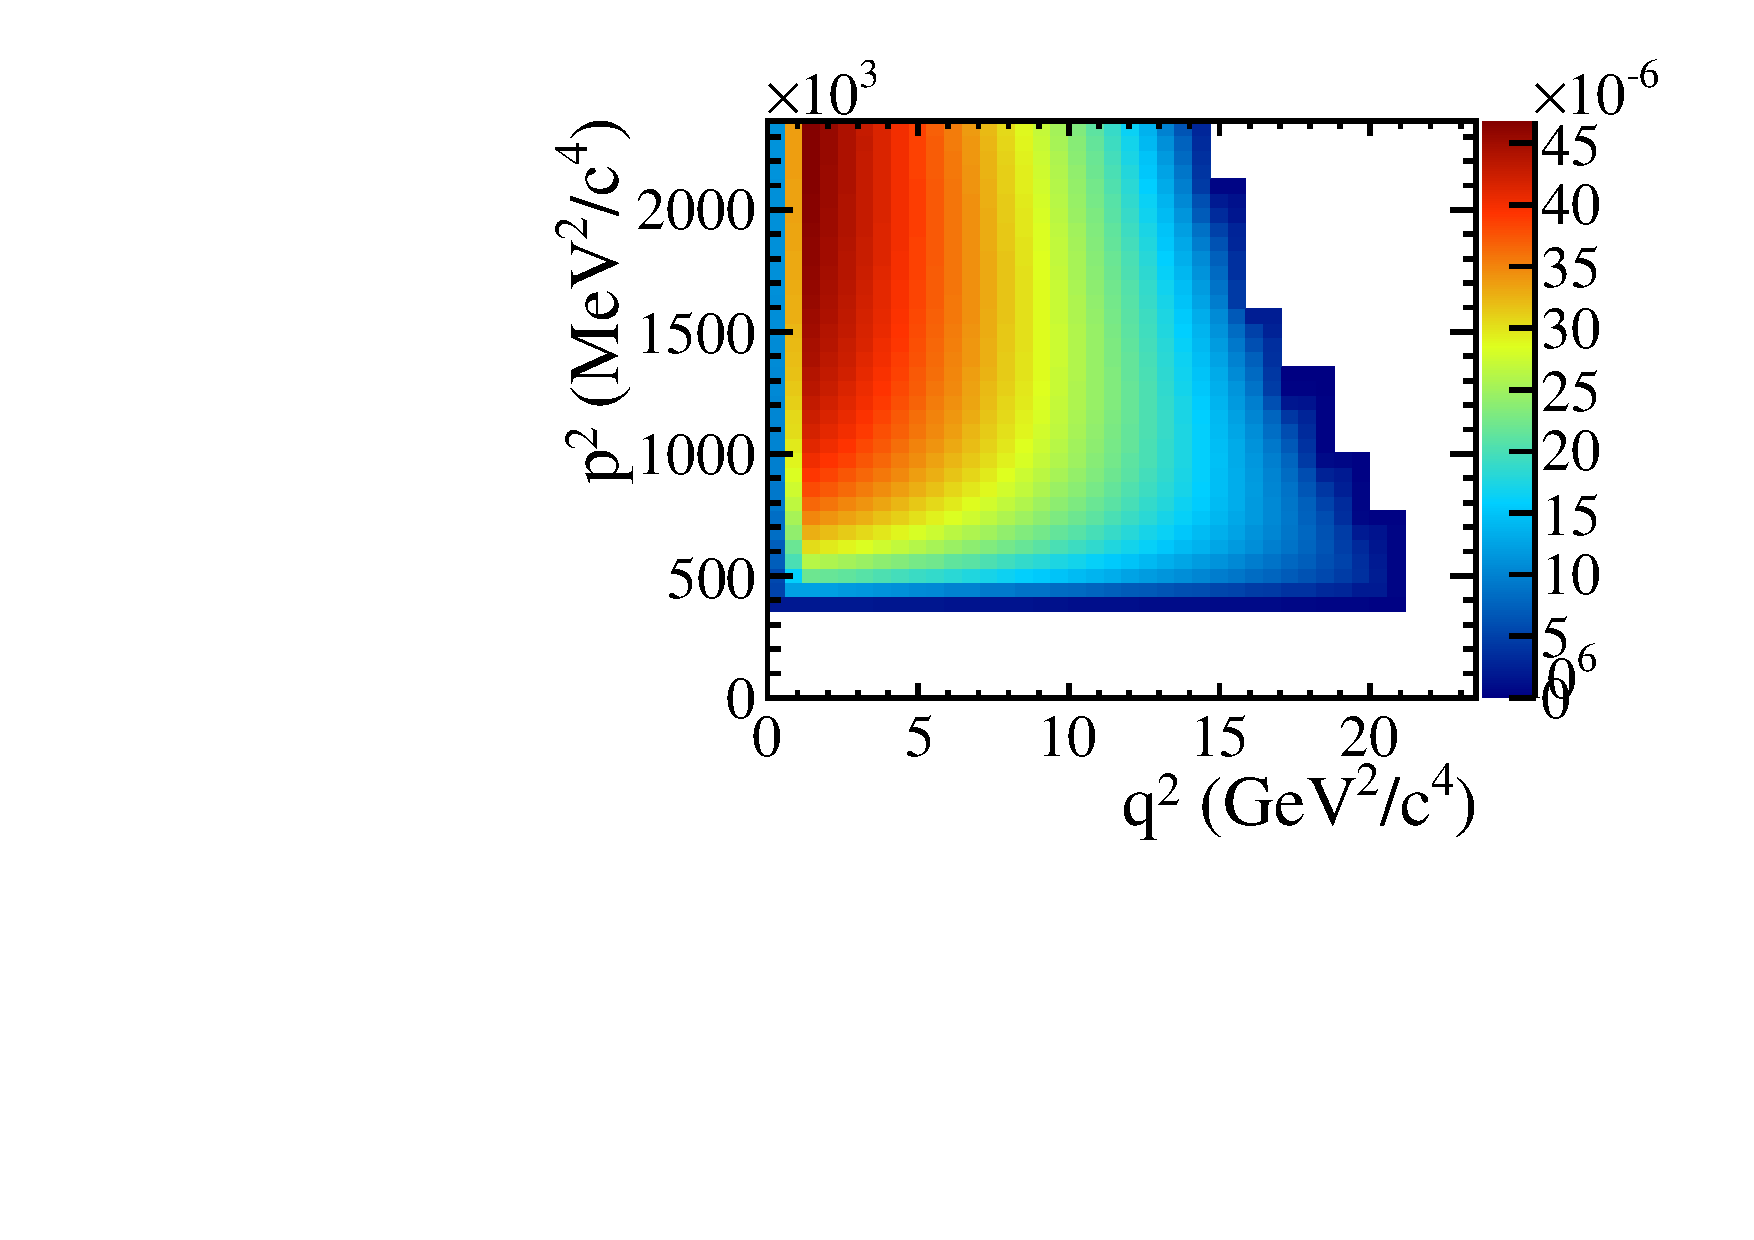
\includegraphics[width=0.48\columnwidth]{chapter6/figs/test_phasespace_psq_qsq.pdf}
\caption[ The phase space for \BdToKpill as a function of \psq and \qsq.   ]
{ The phase space for \BdToKpill as a function of \psq and \qsq. 
The kinematic edge for the high mass \Kstarz states is clearly seen. ~\label{fig:phasespace} }
\end{figure}
The region of S-wave and P-wave interference is mainly at \psq values below $1200^2\mevmevcccc$
 where there is a small reduction in phase space at high \qsq.

\subsection{Propagator functions}
\label{sec:swave:propfunctions}

The propagator for the P-wave is described by a relativistic Breit-Wigner distribution with the amplitude given by
\begin{align}
\label{eq:rbw}
P_1(\psq) = \frac{ m_{\Kstarzo} \Gamma_{\Kstarzo}(\psq)}{ m_{\Kstarzo}^2 - \psq + i \  m_{\Kstarzo} \Gamma_{\Kstarzo}(\psq)} 
\end{align}
where  $m_{\Kstarzo}$ is the resonant mass and 
\begin{align}
\Gamma_{\Kstarzo}(\psq) = \Gamma_{\Kstarzo}^0 \left( \frac{ t }{t_0} \right)^{2J+1} \left( \frac{ m_{\Kstarzo} }{ p } \right) \frac{ B\left(tR_P\right) }{ B\left(t_0R_P\right) }
\end{align}
the running width. Here $t$ is the \Kp momentum in the rest frame of the \kpi system and $t_0$ is t evaluated at the \kpi pole mass.
$B$ is the Blatt-Weisskopf damping factor~\cite{Blatt:628052} with a radius $R_P$.
For P-wave the value of $R_P$ is taken to be $3.0\gev^{-1}$  (from Ref~\cite{Aubert:2008aa}). 
The amplitude can be defined in terms of a phase ($\delta$) through the substitution
\begin{align}
\cot \delta = \frac{  \psq - m_{\Kstarzo}^2 }{  \Gamma_{m_{\Kstarzo}}(\psq) m_{\Kstarzo} }
\end{align}
to give the polar form of the relativistic Breit-Wigner propagator 
\begin{align}
P_1(\psq) =   \frac{1}{\cot\delta - i } 
\end{align}
The LASS parametrisation of the S-wave~\cite{Aston:179353} 
can be used to describe a generic \kpi S-wave.  
In this parametrisation, the S-wave propagator is defined as 
\begin{align}
\label{eq:lass}
P_0(\psq) = \frac{p}{t} \left( \frac{1 }{ \cot\delta_B - i } + e^{2i\delta_B}( \frac{1}{\cot\delta_R - i }) \right)
\end{align}
where the first term is an empirical term from inelastic scattering and the second term is
 the resonant contribution with a phase factor to retain unitarity.
The first phase factor is defined as
\begin{align}
\cot\delta_B = \frac{1}{ta} + \frac{1}{2}rt ,
\end{align}
where $r$ and $a$ are free parameters and $t$ is defined previously,
while the second phase factor describes the $\Kstarzz(1430)$
 through 
\begin{align}
\cot\delta_R = \frac{ \psq - m_{\mathrm{S}}^2 }{ \Gamma_{\mathrm{S}}(\psq) m_{\mathrm{S}}  }.
\end{align}
Here, $m_{\mathrm{S}}$ is the S-wave pole mass and $\Gamma_{\mathrm{S}}$ is the 
running width using the pole mass of the $\Kstarzz(1430)$.
The overall strong phase shift between the results from the LASS scattering experiment and 
measured values for \Bd\to\jpsi\kpi has been found to be consistent with $\pi$~\cite{Aubert:2004cp}. 
The parameters for the \psq spectrum used are given in Table~\ref{tbl:params}.
\begin{table}[tb]
\centering
\caption[ Parameters of the \kpi resonances used to generate toy data sets.    ]
{Parameters of the \kpi resonances used to generate toy data sets. The \Kstar masses and widths 
are taken from Ref.~\cite{PDG2012} and the \Kstarzo Blatt-Weisskopf radius and 
the LASS parameters are taken from Ref.~\cite{Aubert:2008aa}~\label{tbl:params}}
\begin{tabular}{|c|c|c|c|c|c|c|}
\hline
State. & mass & $\Gamma$ & R & $r$ & $a$ & $ \delta_{\mathrm{J}} $ \\
  & (\mev) & $(\mev)$ & ($\gev)^{-1}$ & $(\gev)^{-1}$ & $(\gev)^{-1}$ &  \\
\hline
\Kstarzz & $ 1425  \pm 50 $ & $ 270 \pm 80 $ & $1.0$ & $1.94$ & $1.73$ &  $\pi$ \\
\Kstarzo & $ 894.94  \pm 0.22$ & $ 48.7 \pm 0.8 $ & $3.0$  & \  & \ & 0  \\
\Kstarzt & $ 1432.4  \pm 1.3$ & $ 109 \pm 5 $ & $1.5$  & \  & \ & 0  \\
\hline
\end{tabular}
\end{table} 

\subsection{Angular coefficients}
The angular terms modified by the inclusion of the S-wave are $I_{1,2,4,5,7,8}$ and  
the complete set of angular terms expressed in terms of the spin-dependent amplitudes
are
%Some important features from the angular coefficiencts can by understoof by examination of $I_1^c$, given as
\begin{align}
\label{eq:angularcoeff1}
I_1^c &=  \frac{1}{4\pi} |A_{0L0}|^2 + \frac{3}{4\pi} |A_{1L0}|^2\ctksq + 2 \frac{\sqrt{3}}{4\pi} |A_{0L0}||A_{1L0}|\cos\delta_{0,0}^L \ctk + (L\to R) \frac{}{}  \nonumber \\
I_1^s &= \frac{3}{4} \frac{3}{8\pi} \left( |A_{1L||}|^2 + |A_{1L\bot}|^2 + (L\to R) \right) \frac{}{}\stksq \nonumber   \\
I_2^c &= - I_1^c , \qquad \, I_2^s = \frac{1}{3} I_1^s \nonumber\\ 
I_3 &= \frac{1}{2}  \frac{3}{8\pi}  \left( |A_{1L\bot}|^2 - |A_{1L||}|^2 + (L\to R) \right) \stksq  \frac{}{}\nonumber\\
I_4 &= \frac{1}{\sqrt{2}} \left[  \frac{1}{4\pi}\sqrt{\frac{3}{2}}\Re( A_{0L0}A_{1L||}^{*}) \cos\delta_{0,||}^L \stk  \right. \frac{}{} \nonumber\\
      &+ \left. \frac{3}{4\pi}\sqrt{\frac{1}{2}}\Re( A_{1L0}A_{1L||}^{*})  \stk \ctk  + ( L \to R )  \right] \frac{}{}\nonumber \\
I_5 &= \frac{1}{\sqrt{2}} \left[  \frac{1}{4\pi}\sqrt{\frac{3}{2}}\Re( A_{0L0}A_{1L\bot}^{*}) \cos\delta_{0,\bot}^L \stk  \right. \frac{}{} \nonumber\\
    &+  \left.  \frac{3}{4\pi}\sqrt{\frac{1}{2}}\Re( A_{1L0}A_{1L\bot}^{*})  \stk \ctk  - ( L \to R )  \right] \frac{}{} \\
I_6 &= 2  \frac{3}{8\pi} \left( \Re(A_{1L||}A_{1L\bot}^{*}) - (L\to R) \right) \stksq \frac{}{} \nonumber  \\
I_7 &= \frac{1}{\sqrt{2}} \left[  \frac{1}{4\pi}\sqrt{\frac{3}{2}}\Im( A_{0L0}A_{1L||}^{*}) \cos\delta_{0,||}^L \stk \right. \frac{}{}  \nonumber\\ 
    & + \left.   \frac{3}{4\pi}\sqrt{\frac{1}{2}}\Im( A_{1L0}A_{1L||}^{*})  \stk \ctk   - ( L \to R )  \right] \frac{}{} \nonumber \displaybreak[1]  \\
I_8 &= \frac{1}{\sqrt{2}} \left[  \frac{1}{4\pi}\sqrt{\frac{3}{2}}\Im( A_{0L0}A_{1L\bot}^{*}) \cos\delta_{0,\bot}^L \stk \right. \frac{}{} \nonumber\\
 &  + \left.    \frac{3}{4\pi}\sqrt{\frac{1}{2}}\Im( A_{1L0}A_{1L\bot}^{*})   \stk \ctk  + ( L \to R )  \right]  \frac{}{} \nonumber \\
I_9 &=    \frac{3}{8\pi} \left(  \Im(A_{1L||}A_{1L\bot}^{*}) + (L\to R) \right) \stksq \frac{}{}\nonumber
\end{align}
The interference term of $I_1$ shows how this parametrisation includes the
 strong phase difference between the S- and P-wave state. 
The left handed part of the interference term for $I_1$ can be written as 
\begin{align}
2 |A_{0L0}||A_{1L0}|\cos\delta_{0,0}^L \propto 2\, |M_{0,L,0}||P_0(\psq)||M_{1,L,0}||P_1(\psq)| \cos( \delta_{0,0}^L ) 
\end{align}
where 
\begin{align}
 \delta_{0,0}^L =  \delta_{M_{0L0}} + \delta_{P_0} - \delta_{M_{1L0}} - \delta_{P_1}  .
\end{align}
where $\delta_{M_{JL0}}$ is the phase of the  longitudinal matrix element and 
$\delta_{P_J}$ is the phase of the propagator.
The phases in the interference terms for $I_{4,5,7,8}$ can be similarly defined.
For real matrix elements,~i.e.~nearly true in the Standard Model, the phases are 
equal for both handed interference terms $\delta^L = \delta^R$.
The phase difference between the S-wave and the P-wave propagators can be 
expressed as a single strong phase, $\delta_{\mathrm{S}}$.



\subsection{The \psq spectrum for \BdToKpill}

The \psq spectrum for the  \BdToKpill angular distribution can
 be calculated by summing over the S- and P-waves and integrating 
out the \ctl, \ctk and $\phi$ dependence. This is illustrated in 
Fig.~\ref{fig:psqat6}
\begin{figure}[tb]
\centering
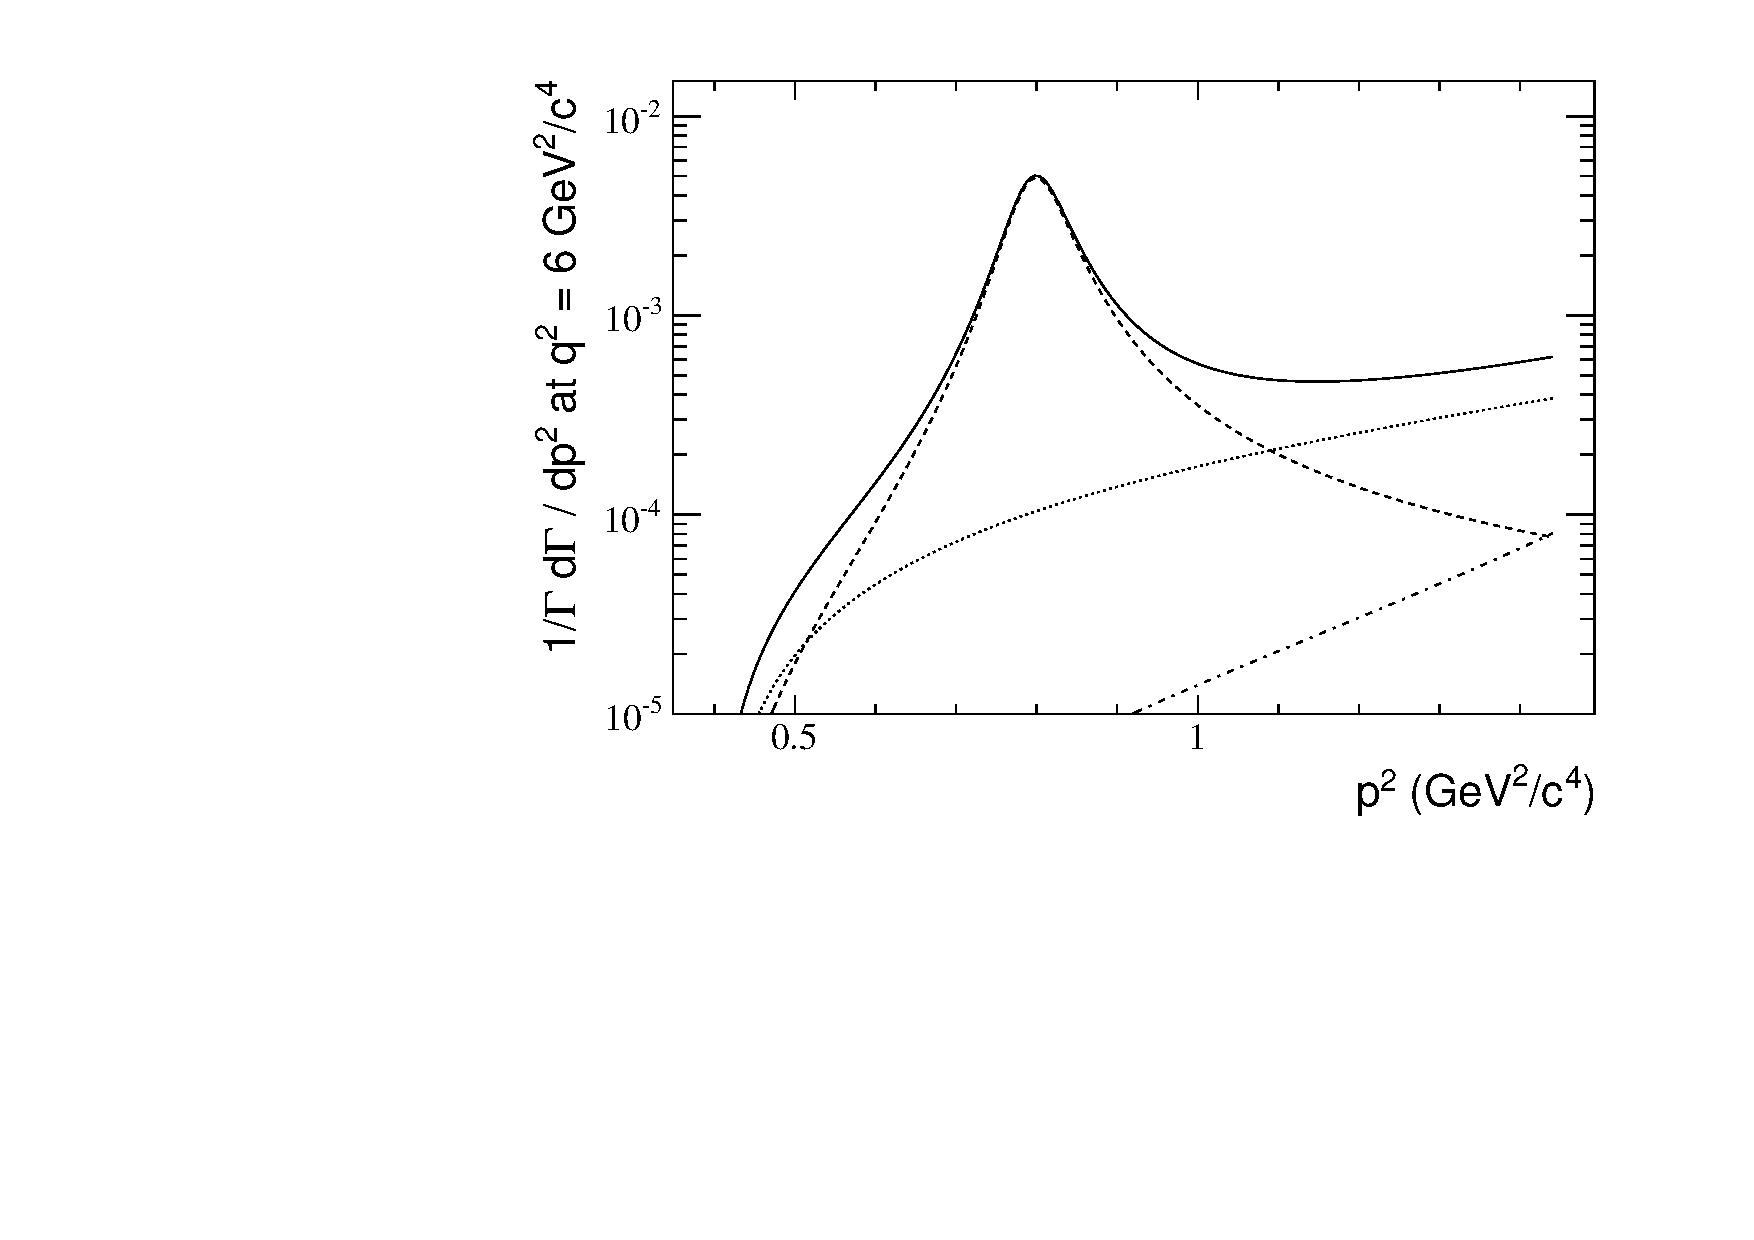
\includegraphics[width=0.66\textwidth]{chapter6/figs/calc_psq_branch_frac_logy.pdf}
\caption[  An illustration of the \psq spectrum for the P-wave (dashed) and the S-wave (dotted).    ]
{ An illustration of the \psq spectrum for the P-wave (dashed) and the S-wave (dotted). 
The total distribution from both states  is the 
solid line. The values were calculated at $q^2 = 6 \gev^2$ by
 integrating out the angular distribution of \BdToKpill using equal 
matrix elements for each state. The S-wave fraction here is 16\% between $800<p<1000 \mev$~\label{fig:psqat6} } 
\end{figure}
where the matrix elements from 
Refs.~\cite{Egede:2008uy,Egede:2010zc} at a \qsq value of $6\gev^2$ are used. 
Here the S-wave amplitude is assumed to be equivalent to the longitudinal P-wave amplitude.
The S-wave fraction in the $800 < p < 1000\mev$ window around the P-wave 
is calculated to be 16\% when using this approximation.
The size of the S-wave fraction, the P-wave fraction and the interference fraction w.r.t the total branching fraction
are given in Fig.~\ref{fig:fracat6}.
\begin{figure}[tb]
\centering
\subfigure[]{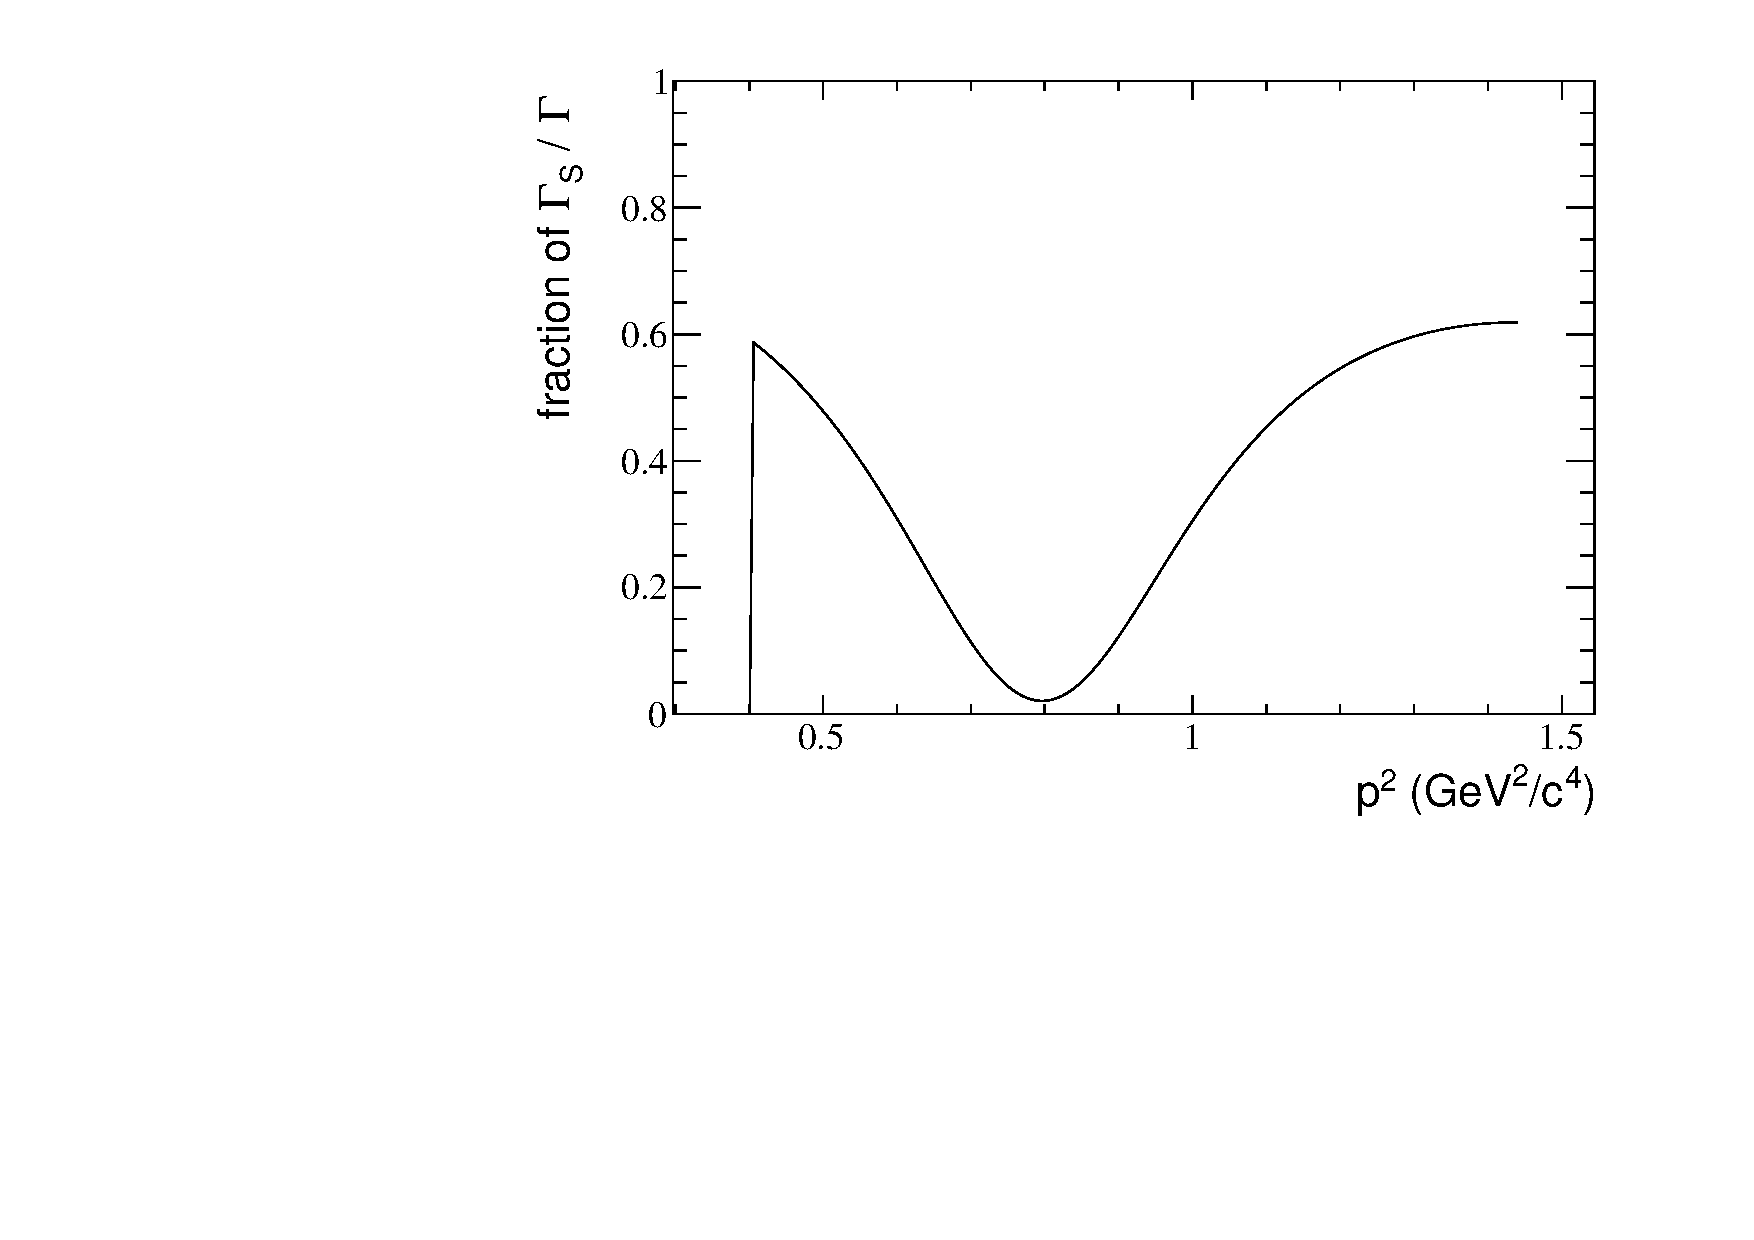
\includegraphics[width=0.48\textwidth]{chapter6/figs/calc_psq_branch_frac_S.pdf}}
\subfigure[]{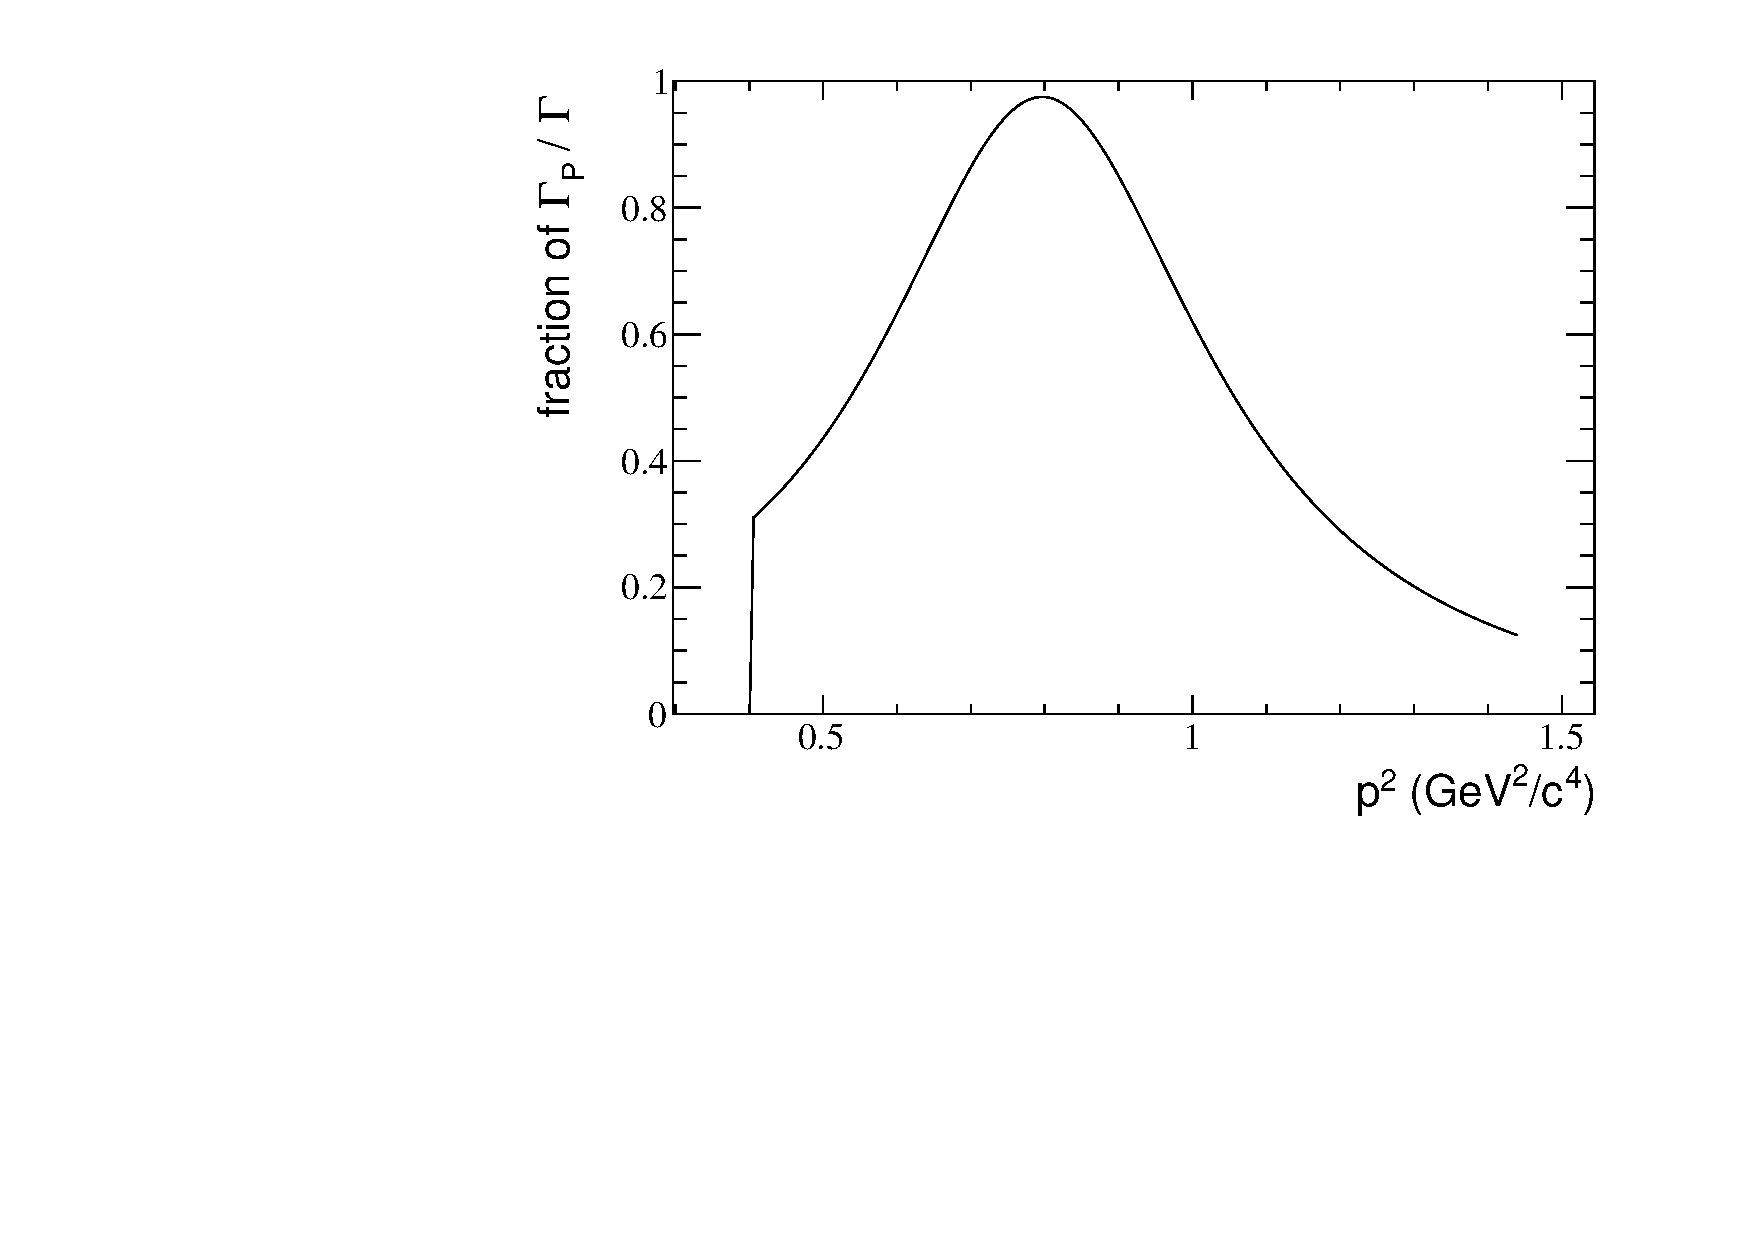
\includegraphics[width=0.48\textwidth]{chapter6/figs/calc_psq_branch_frac_P.pdf}}
\subfigure[]{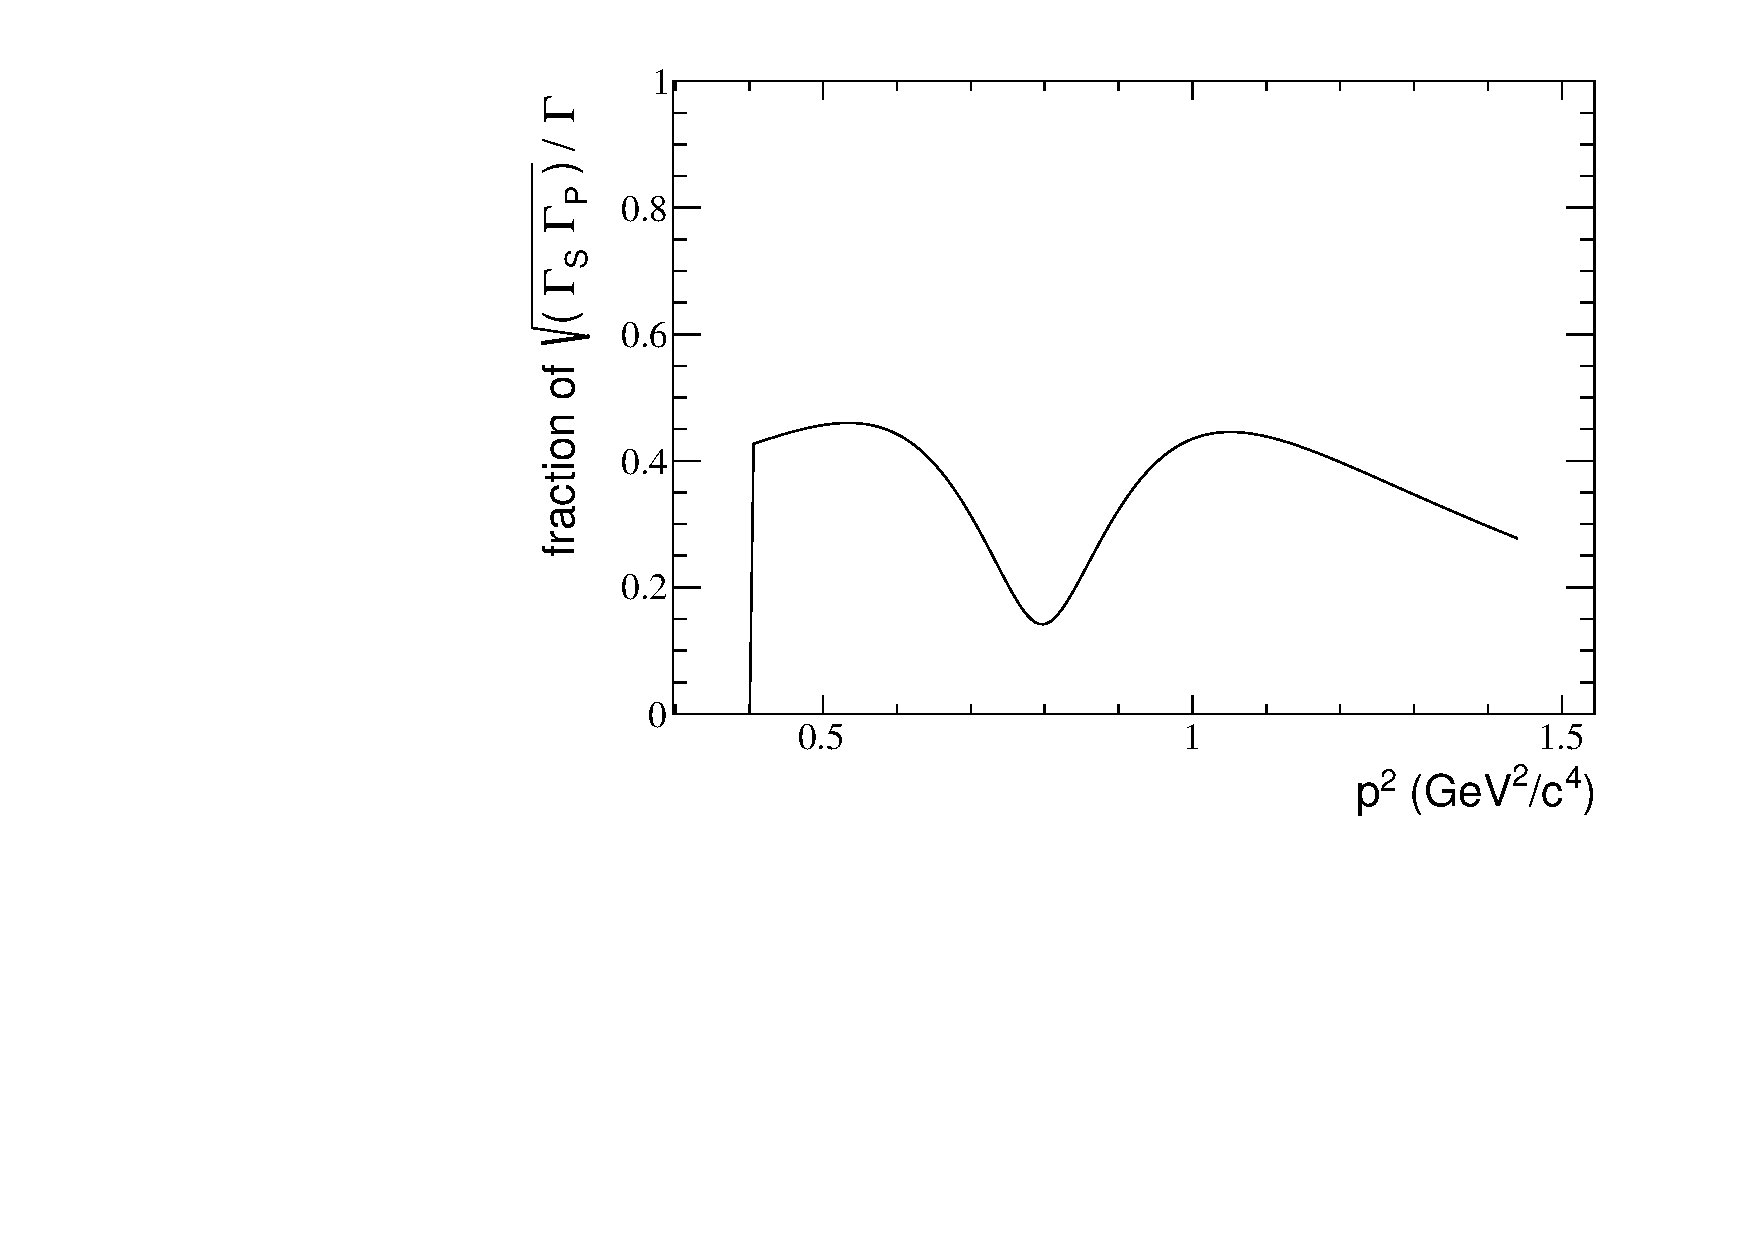
\includegraphics[width=0.48\textwidth]{chapter6/figs/calc_psq_branch_frac_int.pdf}}
\caption[  An illustration of the size of the S-wave, P-wave and S$\leftrightarrow$P-wave
 interference fractions with respect to the total branching fraction. ]
{ An illustration of the size of the S-wave, P-wave and S$\leftrightarrow$P-wave
 interference fractions with respect to the total branching fraction. 
The values were calculated at $q^2 = 6 \gev^2$ by
 integrating out the angular distribution of \BdToKpill using equal 
matrix elements for each state.~\label{fig:fracat6} } 
\end{figure}
As will be seen later there are no interference terms left in the angular distribution after the integral
 over \ctk.


